

After two years of maintenance and upgrades, LHC started the second run phase, also known as \textit{Run2}, in 2015 featuring an increase of the center of mass energy up to 13\tev. The goal of this run is to increase the delivery of particle collisions for physics research, and thereby speed the route to potential new physics. A considerable upgrade program has been planned also for the CMS ad ATLAS detectors, featuring the upgrades of many sub-detectors and software tools. It is possible to study the capabilities that searches for SUSY events in vector boson fusion events have using the new hardware and software setup. This chapter describes a sensitivity study of a SUSY VBF search performed using 13\tev simulated data.

\section{Signal and background samples}

The signal event samples are generated with the \texttt{MadGraph v5.2.1} program \cite{Alwall:2011uj}, considering pair production of gauginos with two associated partons. The signal events are generated requiring a pseudorapidity gap $|\deltaeta| > 4.2$ between the two partons, with $\pt > 30\gev$ for each parton. The signal samples have been generated following all the considerations made for 8\tev analysis for \charginopm = \neutralinotwo masses of 100, 200, 300 and 500\gev. Two are the assumptions made to fix he \stau mass: the fixed-mass and average-mass assumptions. For each of those assumption two different scenarios has been taken into account: the uncompressed mass spectrum and the compressed mass spectrum scenarios.

The Monte Carlo background events used in this study refer to the production run labeled as \texttt{RunIISpring15MiniAODv2} and incorporate the \texttt{CTEQ10} \cite{Dulat:2013hea} parton distribution functions (PDF).The \texttt{POWHEG} and \texttt{MadGraph} generators are interfaced with the \texttt{PYTHIA v8.5.12} \cite{Sjostrand:2006za} program, which is used in the matching between the matrix elements, the parton shower, and the hadronization processes. 

All the Monte Carlo samples are stored in a new format called \texttt{miniAOD} \cite{bib:WorkBookMiniAOD}. This format is an updated version of the previously used one and includes the new CMS reconstruction features developed between the time of the original analysis and the starting of Run2. A comprehensive list of all the samples used in this study is listed in \autoref{sec::sampleslist_13tev}.

\section{Object reconstruction}

The upgrade plan commissioned for the CMS detectior translates also into an updated version of the physical object definition used for this study with respect to the one used in the 8\tev analysis.

The \hadtau object reconstruction went through a major update with the introduction of new isolation and decay mode discriminators and electron veto \cite{bib:TauID_13tev}. Its reconstruction has been commissioned for $\pt > 20$\gev in all $\eta$ ranges. Using the specifications suggested by the Tau POG, an increase of the overall TauID efficiency of about 10\% for loose isolated \hadtau with respect to the 8\tev specifications is achieved, with the recontructon efficiency going up to 71\% for $Z \longrightarrow\tau\tau$ events\cite{bib:TauID_13tev}. A detailed list of the \hadtau object selection can be found in Table \ref{table:tauobjdefinition_13TeV}. 

The Jet object definition remained unchanged with respect to the one used in the 8\tev analysis.  

With Run 2 the experiment gains access to a new trigger list. The aim is to use a trigger that is exclusively making an online selection on the dijet object kinematic properties. Differently with respect to the 8\tev trigger version, this trigger cannot be seeded by a level one trigger based on \met. The drop of all online selections over the \hadtau properties leads to some important advantages. First, it is possible to have a lower \hadtau \pt selection. Second, it is possible to go from a 1-prong to a 3-prong decay selection since this stringent requirement is not a part of any level 1 trigger seed. 

The b-tag object reconstruction has an updated discriminator as suggested by the POG \cite{bib:BJetID_13tev}.

\section{Cross section limit studies}

The aim of this study is to optimize the event cuts is order to exclude signal at the lowest cross section measurable. A cross section limit is made by setting the so called significance $\alpha$ to:

\begin{equation}
\alpha = 2
\label{eq::significance_xsec_limit}
\end{equation}

There are several definitions of significance $\alpha$ available in literature, however the one picked for this 13\tev study is a frequentist definition based on completely standard concepts\cite{Punzi:2003bu} which is generally applicable, and has a very clear interpretation. It is particularly suitable for optimization, being independent of a-priori expectations about the presence of a signal, thus allowing the determination of a single set of cuts that is optimal both for setting limits and for making a discovery. The definition of sensitivity is:

\begin{equation}
\alpha = \dfrac{S}{\dfrac{a}{2} + \sqrt{B + \left( \dfrac{B}{2}\right)^{2}}}
\label{eq::punzi_formula}
\end{equation}

with $a$ the confidence level expressed in terms of $\sigma$, and $S$ and $B$ the number of signal and background vents for a given selection. One of the most important features of \autoref{eq::punzi_formula} that it is non-diverging in case of $B = 0$.

The number of signal events can be defined as:

\begin{equation}
S = \epsilon \cdot \sigma_{sec} \cdot L
\label{eq::punzi_signal_events}
\end{equation}

where $\epsilon$ is the efficiency for a given selection criteria, $\sigma_{sec}$ the cross section of the signal process considered and $L$ the luminosity given by the experiment. Is it possible now to define the efficiency $\epsilon$ as function of variables used in the analysis event selection. Three of the most important variables in the 8\tev analysis has been chosen for this study: $\pt(\hadtau)$, \met and $m_{jj}$. The definition of $\epsilon$ in \autoref{eq::punzi_signal_events} now becomes:

\begin{equation}
\epsilon^{signal} ( \pt(\hadtau) , m_{jj} ,  \met ) = \dfrac{N^{signal}_{passed}(\pt(\hadtau) , m_{jj} ,  \met)}{N^{signal}_{total}}
\label{eq::punzi_efficiency}
\end{equation}

where $N^{signal}_{passed}$ is the number of signal events passing the selection criteria as a function of the chosen variables and $N^{signal}_{total}$ is the total number of signal events. It is easy to notice that by fixing the significance value as shown on \autoref{eq::significance_xsec_limit} the cross section $\sigma_{sec}$ in \autoref{eq::punzi_signal_events} becomes indeed the cross-section limit $\sigma^{lim}_{sec}$. After merging both \autoref{eq::punzi_signal_events} and \autoref{eq::punzi_efficiency} the cross section limit $\sigma^{lim}_{sec}$ is defined as:
	
\begin{equation}
\sigma^{lim}_{sec}( \pt(\hadtau) , m_{jj} ,  \met ) = \dfrac{\alpha \cdot\left(\dfrac{a}{2} + \sqrt{B( \pt(\hadtau) , m_{jj} ,  \met ) + (0.5 \cdot B( \pt(\hadtau) , m_{jj} ,  \met ))^{2}}\right)}{\epsilon^{signal} ( \pt(\hadtau) , m_{jj} ,  \met ) \cdot L}
\label{eq::xsec_lim}
\end{equation}



\subsection{Event selection}
\label{subsec::event_sel_13tev}

The values for $\epsilon^{signal}$ and $B$ are directly taken from the signal and background samples listed in \autoref{sec::sampleslist_13tev}, on which the event selection has been applied. The idea of this 13\tev study is to be as close as possible to the one done in 8\tev, therefore the event selection is very similar to the one described in \autoref{sec:eventselection}.

As previously mentioned the event selection for this study is a function of the reconstructed tau \pt , \met and the di-jet candidate invariant mass $m_{jj}$, therefore those cuts are considered as free variables in the event selection. 

The uncertainties on the official 13\tev trigger list and on how good are those triggers simulated in Monte Carlo lead to the decision of removing the trigger requirement in the event selection. In case this study will use 13\tev data it is useful to notice that a choice of a VBF-selection-seeded trigger will lead to an online selection over the di-jet canditates invariant mass $m_{jj}$.

The di-jet \deltaeta cut has been removed due to its strong correlation to the di-jet canditates invariant mass $m_{jj}$ as shown in the 8\tev study \cite{Khachatryan:2015kxa}.

For better visualization and understanding, all the selection criteria are summarized below:

\begin{itemize}
	\item \textbf{Central selection}
	\begin{itemize}
		\item two one-prong hadronically decaying $\tau$ with $\pt = 20,25,30,35,40,45\gev$
		\item $0 < \met < 240\gev$
		\item at least two jets with $p_{T}^{jet}\geq30~$\gev, $|\eta_{jet}|\leq5$ and loose jetID
		\item $\Delta R(jet,\tau)\geq0.3$
		\item b-tag veto
	\end{itemize}
	\item \textbf{VBF selection}
	\begin{itemize}
		\item $\text{sign}(\eta^{jet 1}\cdot\eta^{jet 2})=-1$
		\item $ 0 < \mjj < 2500\gev$
	\end{itemize}
\end{itemize}

\subsection{Background estimation}

Similar to the analysis at 8\tev, the largest challenge for this study is to determine the number of background events in the signal region. As described in \autoref{sec::bg_contributions}, the main background contribution is coming from QCD events. The remaining background contributions are considered negligible. Even though this study is characterized by a loosening of the selection cuts with respect to the previous analysis, the limited statistics of the Monte Carlo samples used gives a very scarce number of selected events. The problem of a limited statistics is solved by estimating the number of background events in the signal region through a two-fold ABCD method. It involves the usage of two distinct correction factors in order to gradually convert the number of background events, taken from a starting control region with looser cuts, into the signal region ones. This method is defined under the same assumptions made for the 8\tev analysis, listed in \autoref{sec:bgestimation}.

Bearing in mind the idea of developing a method similar to the one used for 8\tev, the regions are defined by two distinct variables: the isolation of the di-tau candidates and the inversion of the VBF cuts. There are three regions defined for this method. The signal region, also called SR, is defined as the region fulfilling all the cuts listed in \autoref{subsec::event_sel_13tev}. Control region two, also called CR2, has the same selection as the one for the signal region but requires the inversion of the VBF-related cuts. Finally control region three, also called CR3, has the same selection as CR2 but requires the di-tau candidates to have a Loose isolated and a non-isolated \hadtau.

\begin{figure}[tbh!]
	\centering
	\begin{tabular}{cc}
		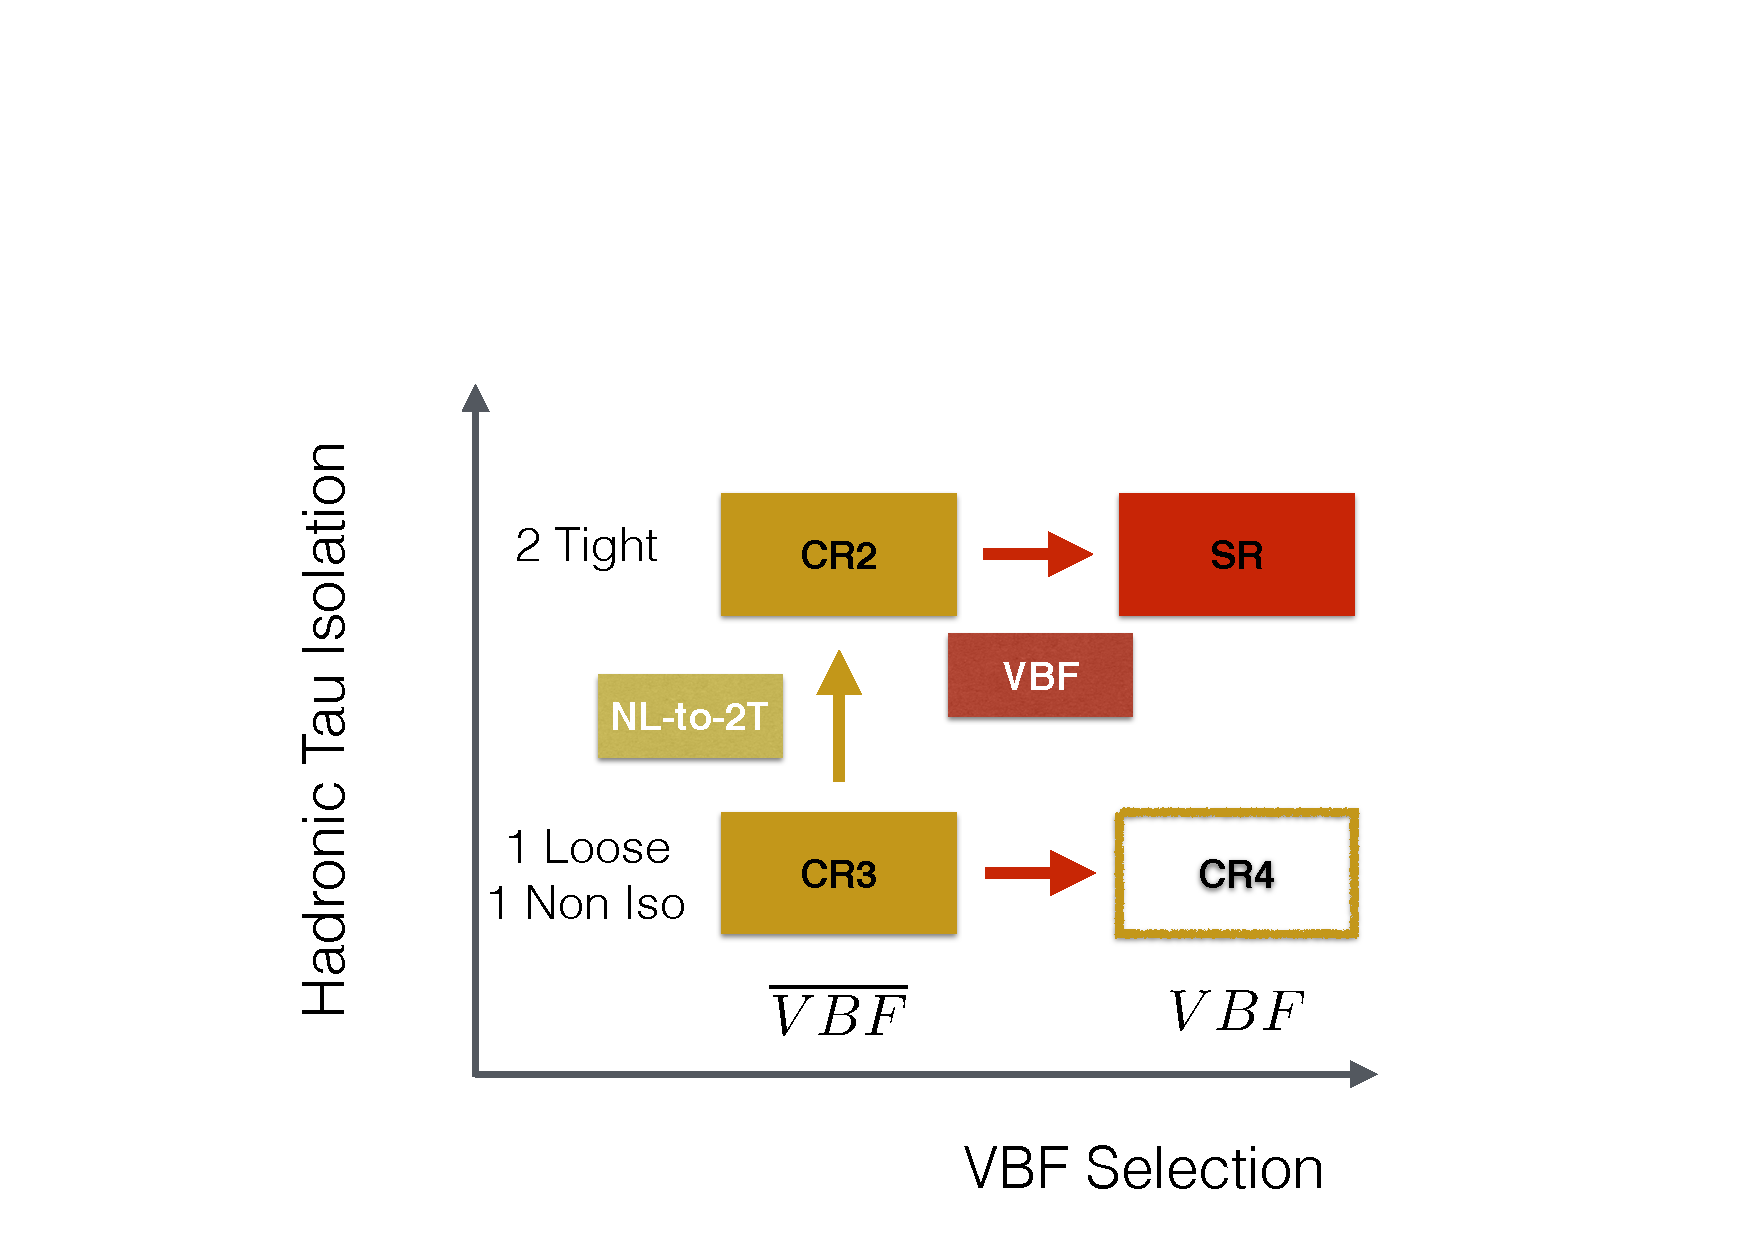
\includegraphics[width=0.75\textwidth]{PLOTS/diTauHadLSotherPlots/controlregions13TeV.pdf}
	\end{tabular}
	\caption{Definition of Signal and Control Regions using different $\hadtau$ isolation criteria and VBF selection.}
	\label{fig:crs_13tev}
\end{figure}

As previously mentioned, two conversion factors are used in this method. The first factor, named "\textit{NL-to-2T}" or "\textit{None-Loose to two Tight}", allows to convert the number of selected events from CR3 to CR2. This factor is derived from a study over the same QCD sample where the event population is high by only requiring at least four reconstructed jets in the event, and is defined as:

\begin{equation}
\text{NLto2T} = A \cdot B
\end{equation}

where $A$ and $B$ are ratios. Further, $A$ has as denominator the number of events with at least four jets where at least one of these jets is matched with a loose isolated \hadtau. In case this matched \hadtau is also tight isolated the events are counted in the numerator:

\begin{equation}
A = \dfrac{N_{events}(\text{the matched }\hadtau\text{ is also tight isolated })}{N_{events}(\leq 1\text{jet matched to loose }\hadtau)}
\end{equation}

The definition of $B$ is equal to $A$ with the only difference that the \hadtau matched to a jet in the denominator is non-isolated:

\begin{equation}
B = \dfrac{N_{events}(\text{the matched }\hadtau\text{ is also tight isolated })}{N_{events}(\leq 1\text{jet matched to non-isolated }\hadtau)}
\end{equation}

The second conversion factor is identical to the VBF conversion factor defined in \autoref{sec:bgestimation} with the only difference of the updated version of the VBF cuts for the 13\tev study:

\begin{equation}
\text{VBF} = \frac{\epsilon^{QCD}_{VBF}}{1 - \epsilon^{QCD}_{VBF}}
\end{equation}

where $\epsilon^{QCD}_{VBF}$ is previously defined in \autoref{eq:vbfeff}. 

Finally the number of predicted events in the signal region is:

\begin{equation}
B = N^{QCD}_{SR} = N^{MC}_{CR3}  \cdot \text{NLto2T} \cdot \text{VBF}
\label{eq::qcdbgpred_13tev}
\end{equation}

A representation of the regions and the conversion factor used in this two-fold ABCD method is shown in \autoref{fig:crs_13tev}.

\subsection{Systematic and statistical uncertainties}

As in the 8\tev analysis, two different sources of systematics have been taken into account for this study. 

The first source is the uncertainty originating from the simulated samples. Following the strategy used in the previous analysis this systematic uncertainty is estimated from the variation on the cross-section limit result after considering a $\pm 50\%$ variation of the Monte Carlo statistics.

The second source of the uncertainty is the instability on the VBF efficiency $\epsilon^{QCD}_{VBF}$ over different \hadtau isolation regions. Again, this uncertainty is calculated by taking into account the maximal variation of the VBF conversion factor in the previously defined control regions, CR2 and CR3.

\section{Results}

The definition of the cross-section limit $\sigma^{lim}_{sec}$, as given in \autoref{eq::xsec_lim}, allows a scan in a three-dimensional space defined by the variables $\pt(\hadtau)$ , \mjj and \met. The minimum cross-section limit found by the scan gives the optimal event selection cuts for each of the available signal benchmark points. The distribution of the most important analysis variables are shown in \autoref{fig::crplots1_Taui2TightIso_13tev_results}, \autoref{fig::crplots2_Taui2TightIso_13tev_results}, \autoref{fig::crplots3_Taui2TightIso_13tev_results} and \autoref{fig::crplots4_Taui2TightIso_13tev_results}; for this purpose the cuts over the study variables $\pt(\hadtau)$, \mjj and \met have been removed. 

For an easier reading over the results of the cross-section limit study, it is possible to simplify the three-dimensional problem in a "\textit{two plus one}" dimensional one. Following this approach, the cross-section limits are calculated and shown in a two-dimensional plot defined in bins of \mjj and \met. This process is then repeated for each of the chosen $\pt(\hadtau)$ cuts.

\begin{figure}[tbh!]
	\centering
	\begin{tabular}{cc}
		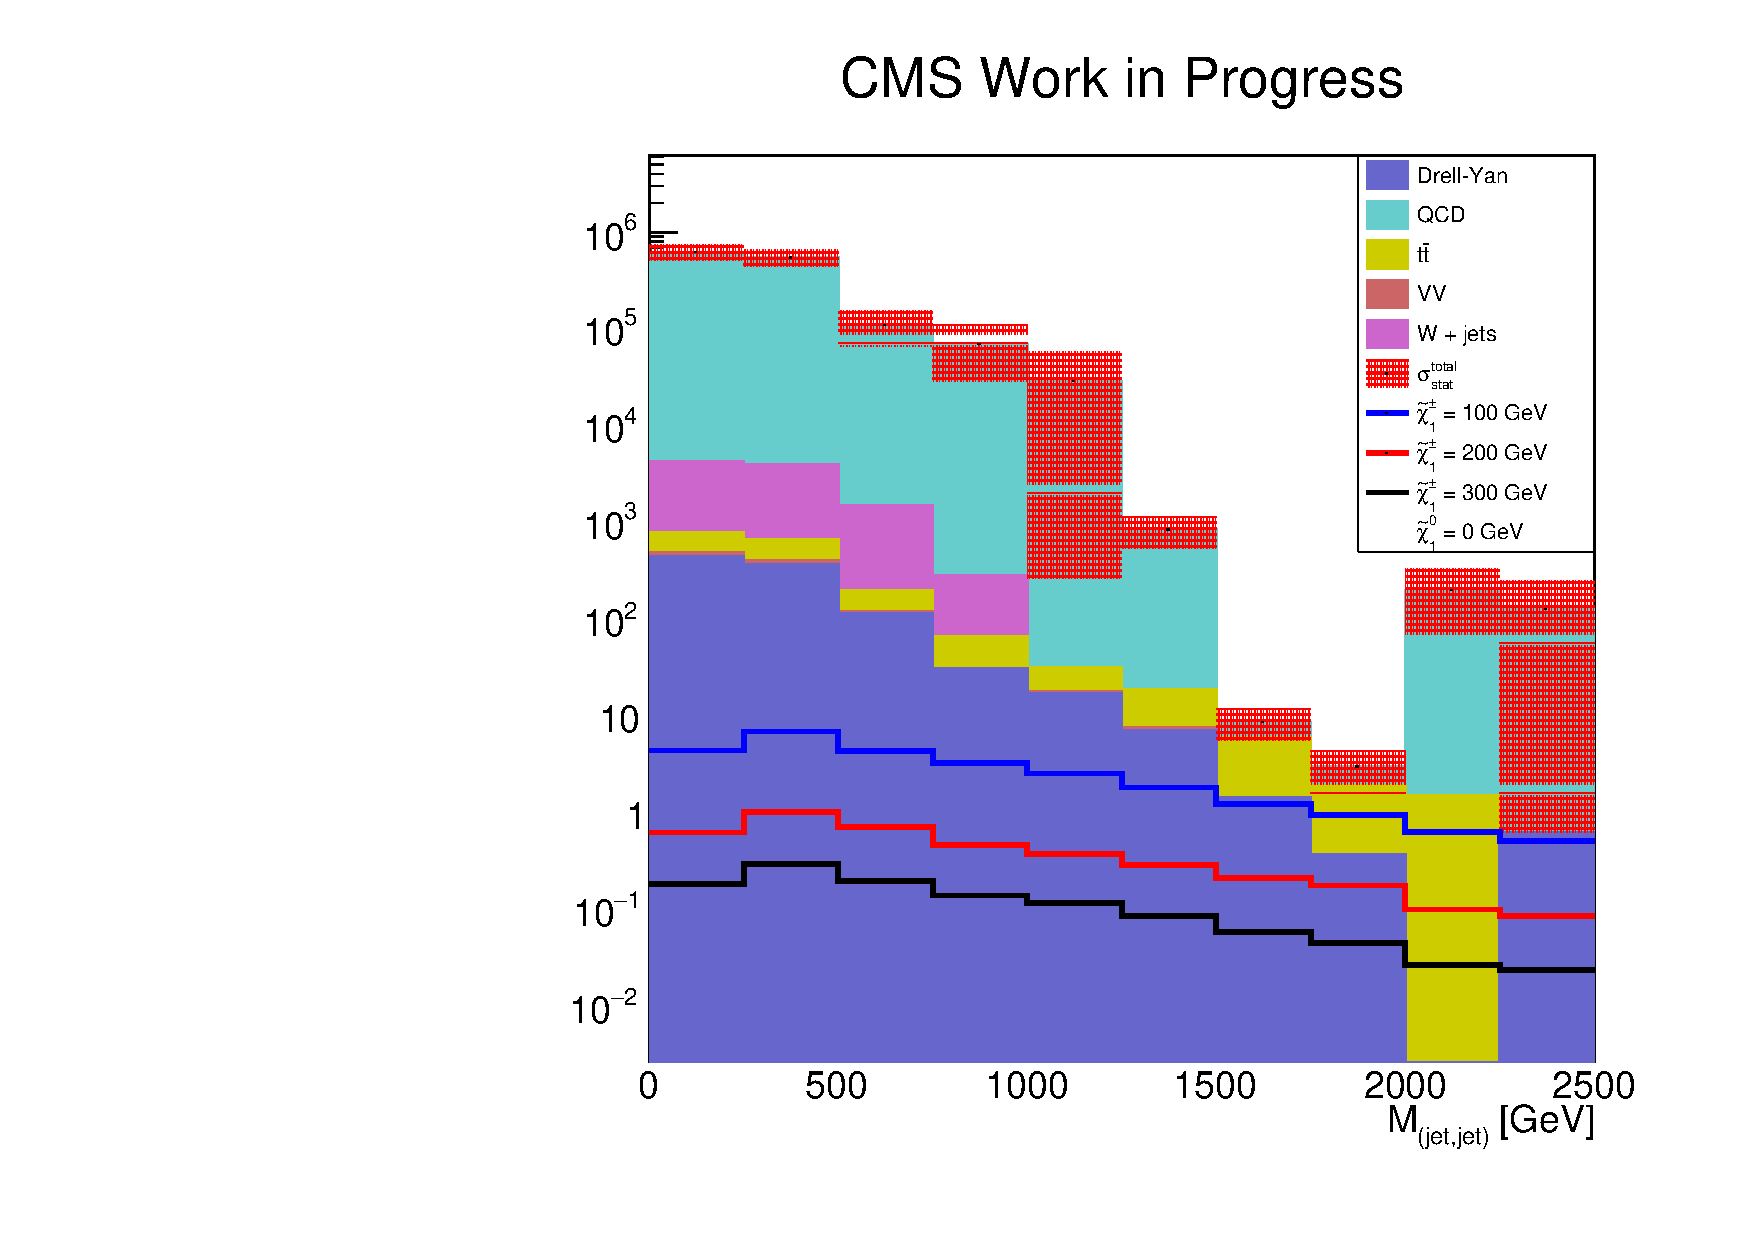
\includegraphics[width=0.5\textwidth]{analysis/pics/h_dijetinvariantmass_Taui2TightIso.pdf}
		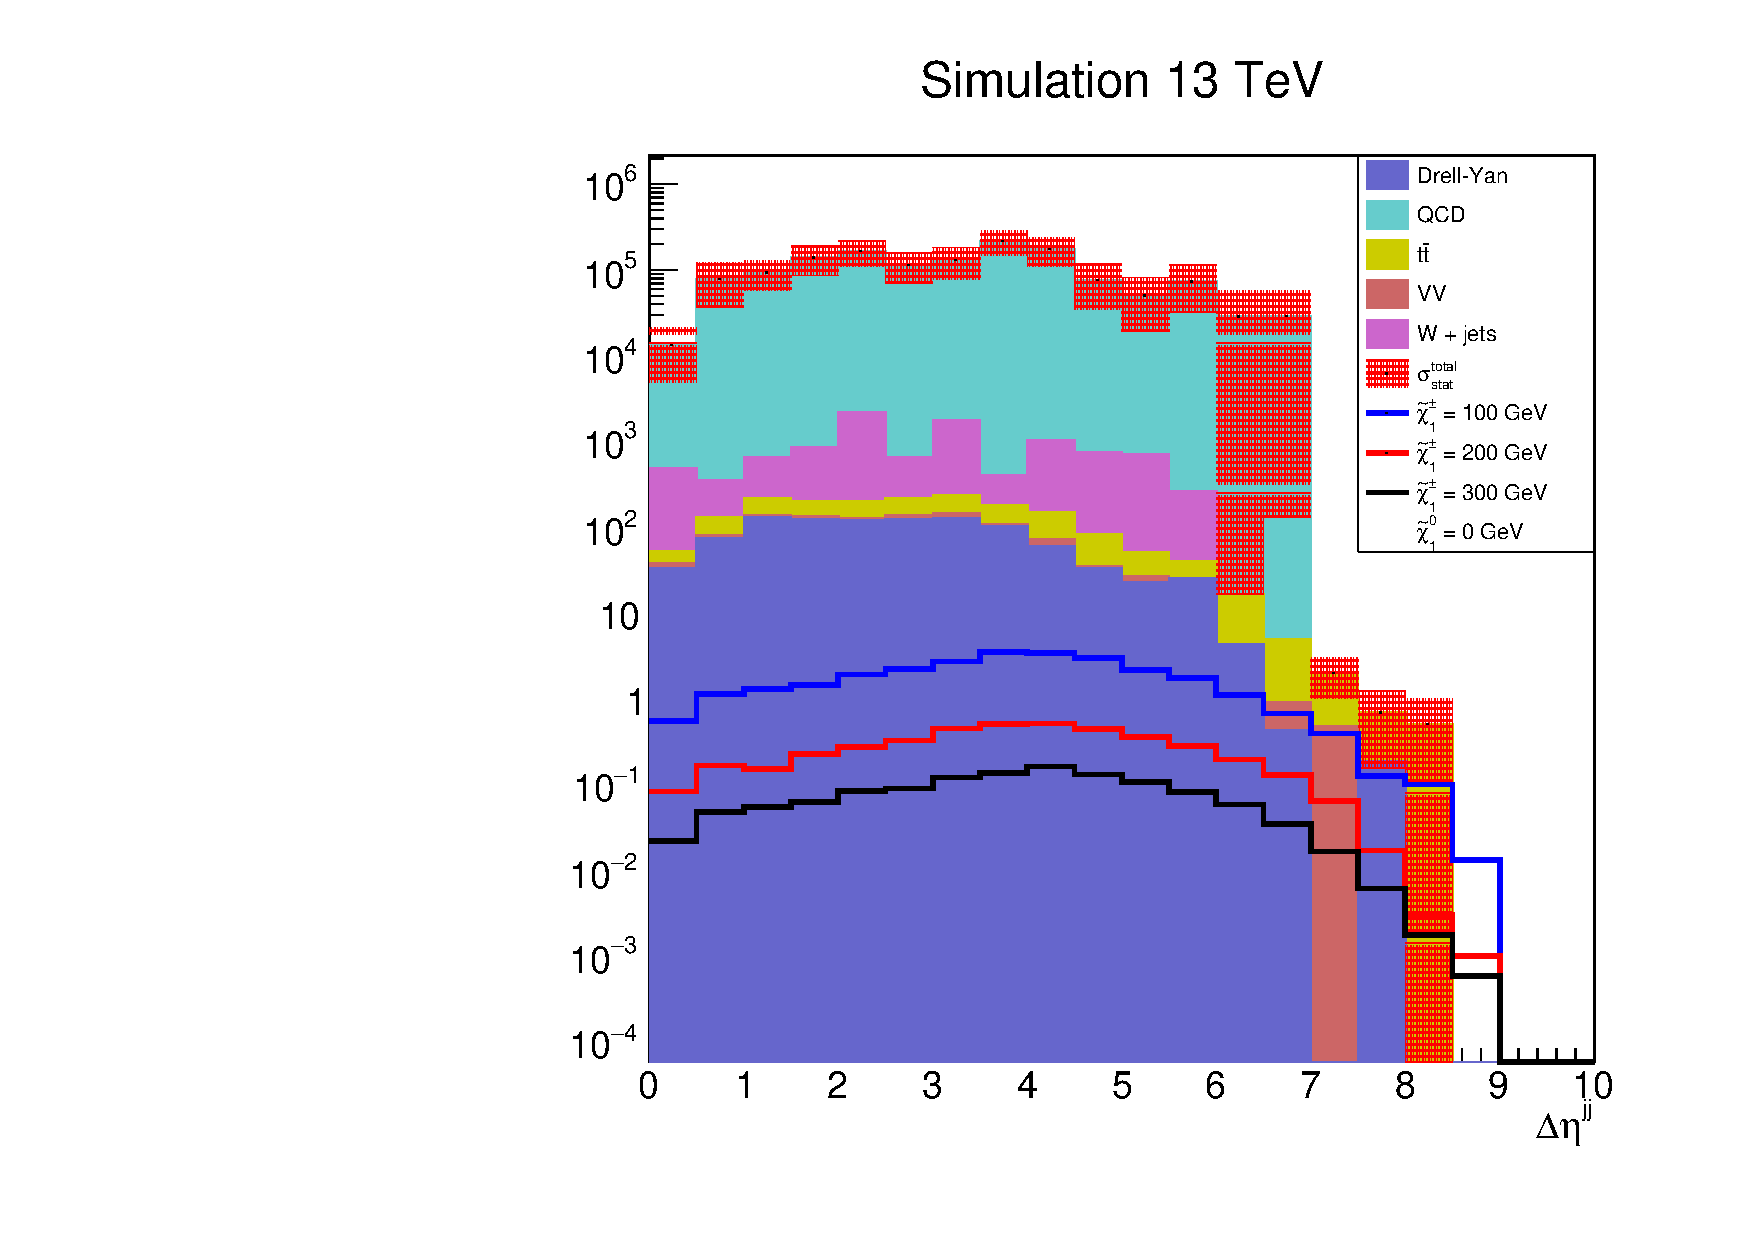
\includegraphics[width=0.5\textwidth]{analysis/pics/h_dijetdeltaeta_Taui2TightIso.pdf} 		
	\end{tabular}
	\caption{(Left) Di-jet invariant mass distribution and (Right) and Di-jet \deltaeta distribution of selected signal and all MC background samples in signal region.}
	\label{fig::crplots1_Taui2TightIso_13tev_results}
\end{figure}

\begin{figure}[tbh!]
	\centering
	\begin{tabular}{cc}
		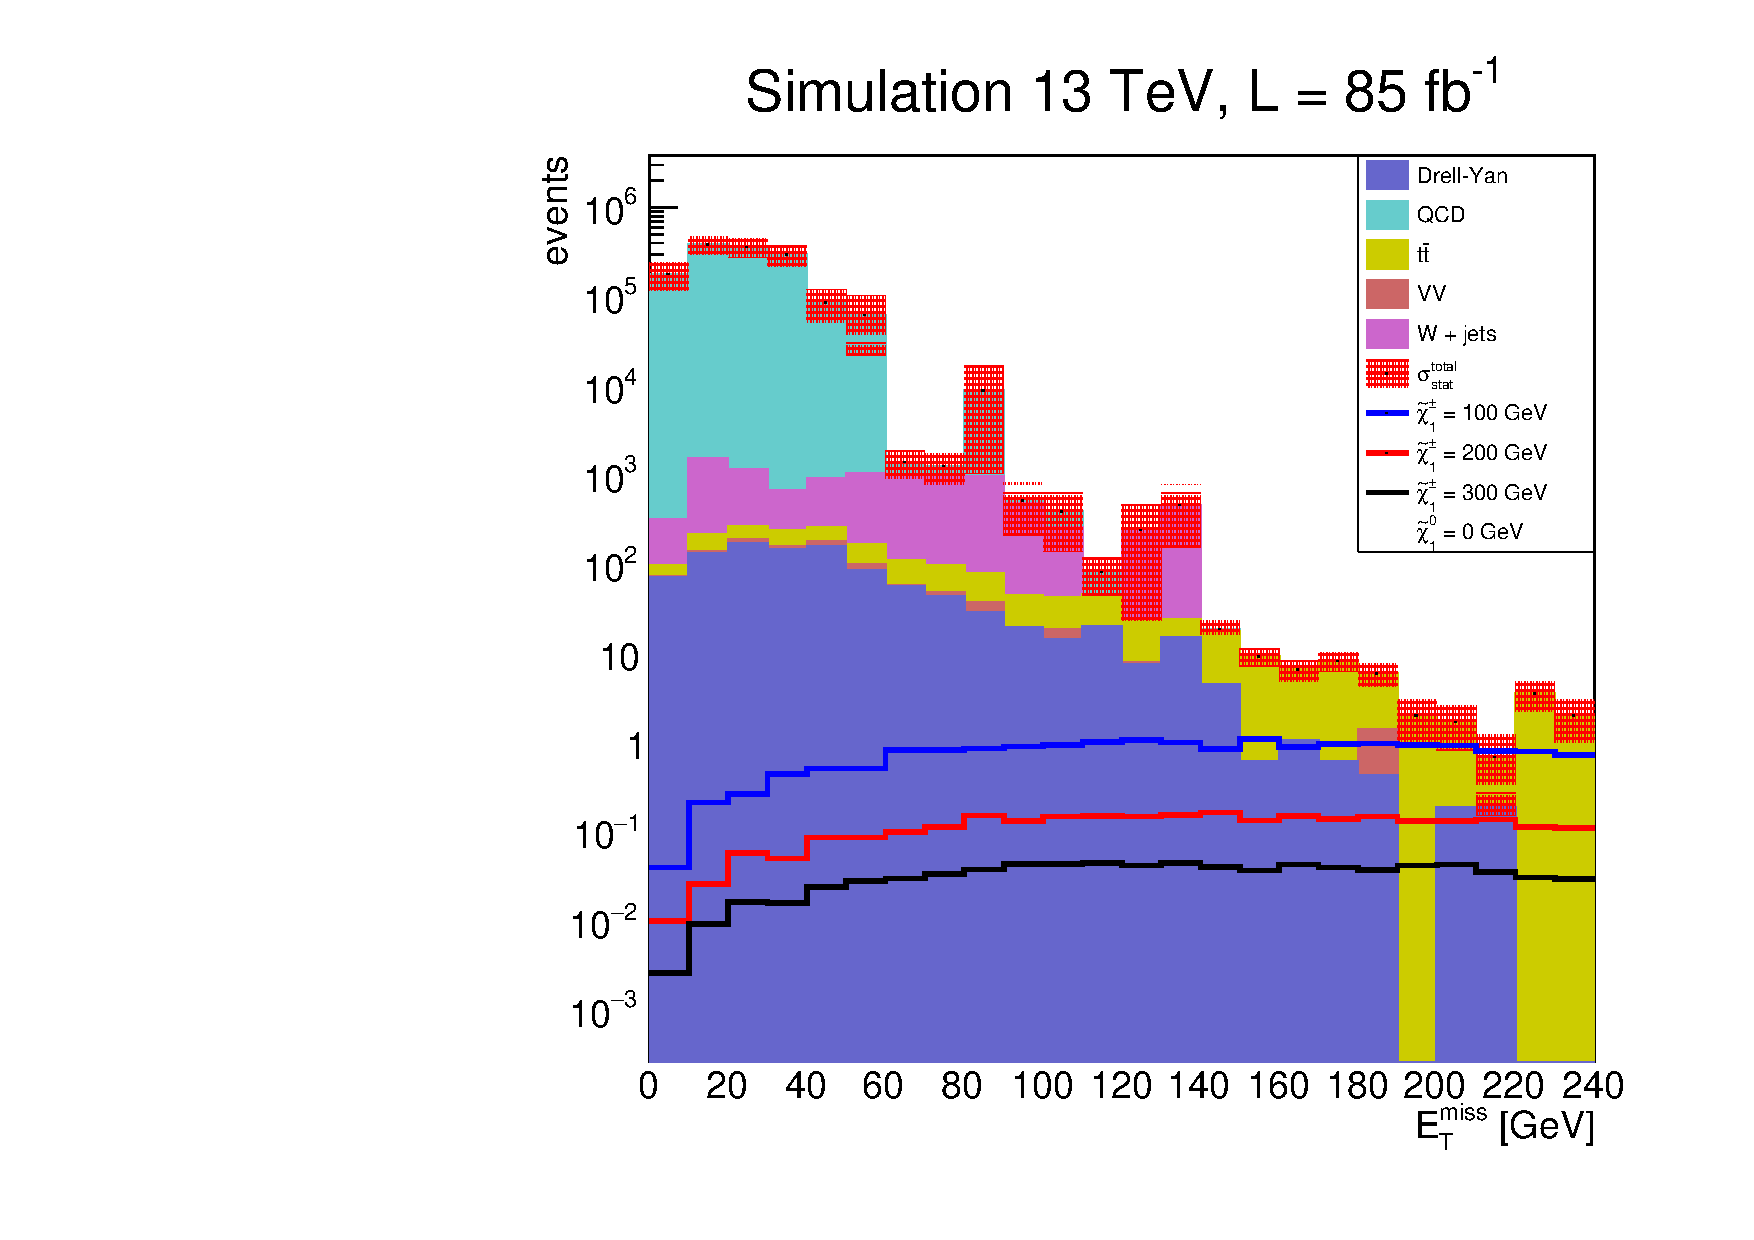
\includegraphics[width=0.5\textwidth]{analysis/pics/h_met_Taui2TightIso.pdf}
		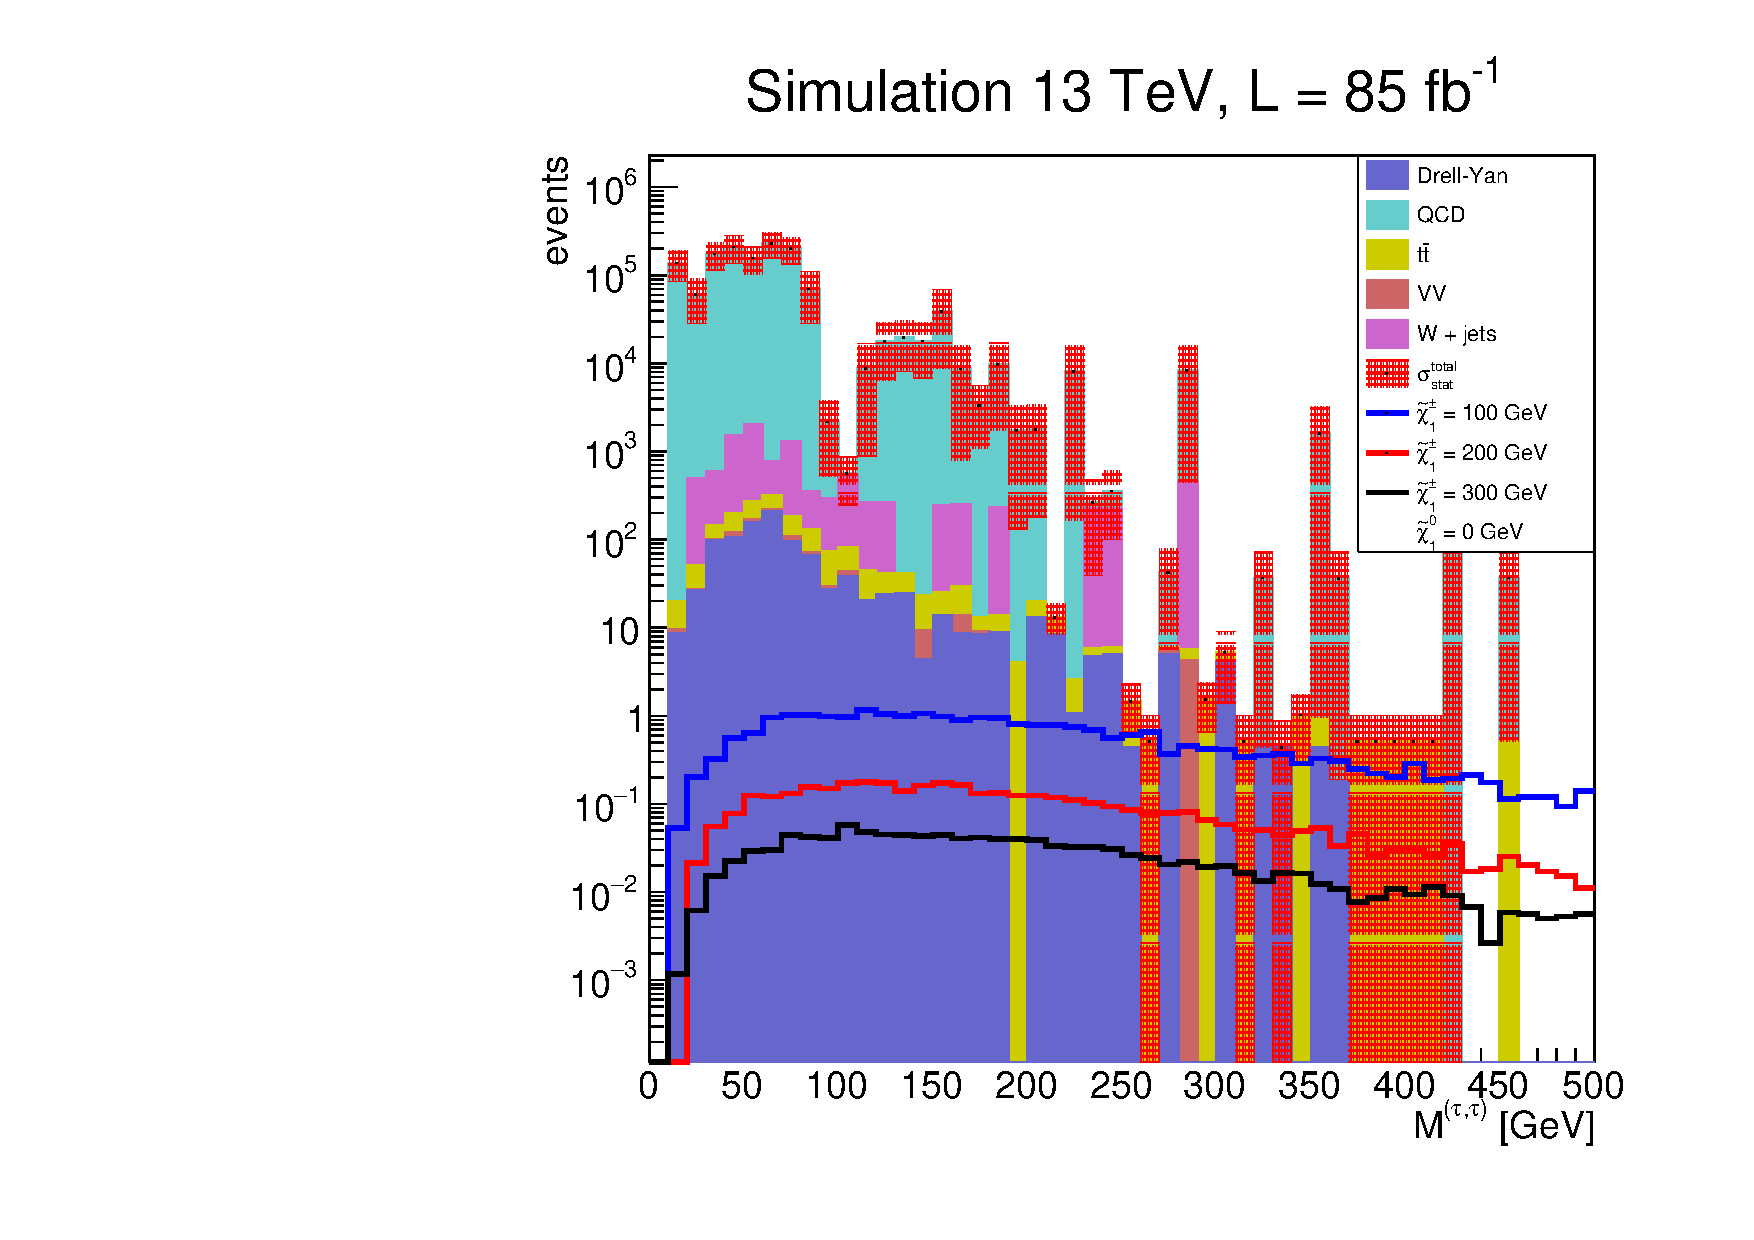
\includegraphics[width=0.5\textwidth]{analysis/pics/h_ditauinvariantmass_Taui2TightIso.pdf} 		
	\end{tabular}
	\caption{(Left) \met distribution and (Right) and Di-\hadtau invariant mass distribution of selected signal and all MC background samples in signal region.}
	\label{fig::crplots2_Taui2TightIso_13tev_results}
\end{figure}


\begin{figure}[tbh!]
	\centering
	\begin{tabular}{cc}
		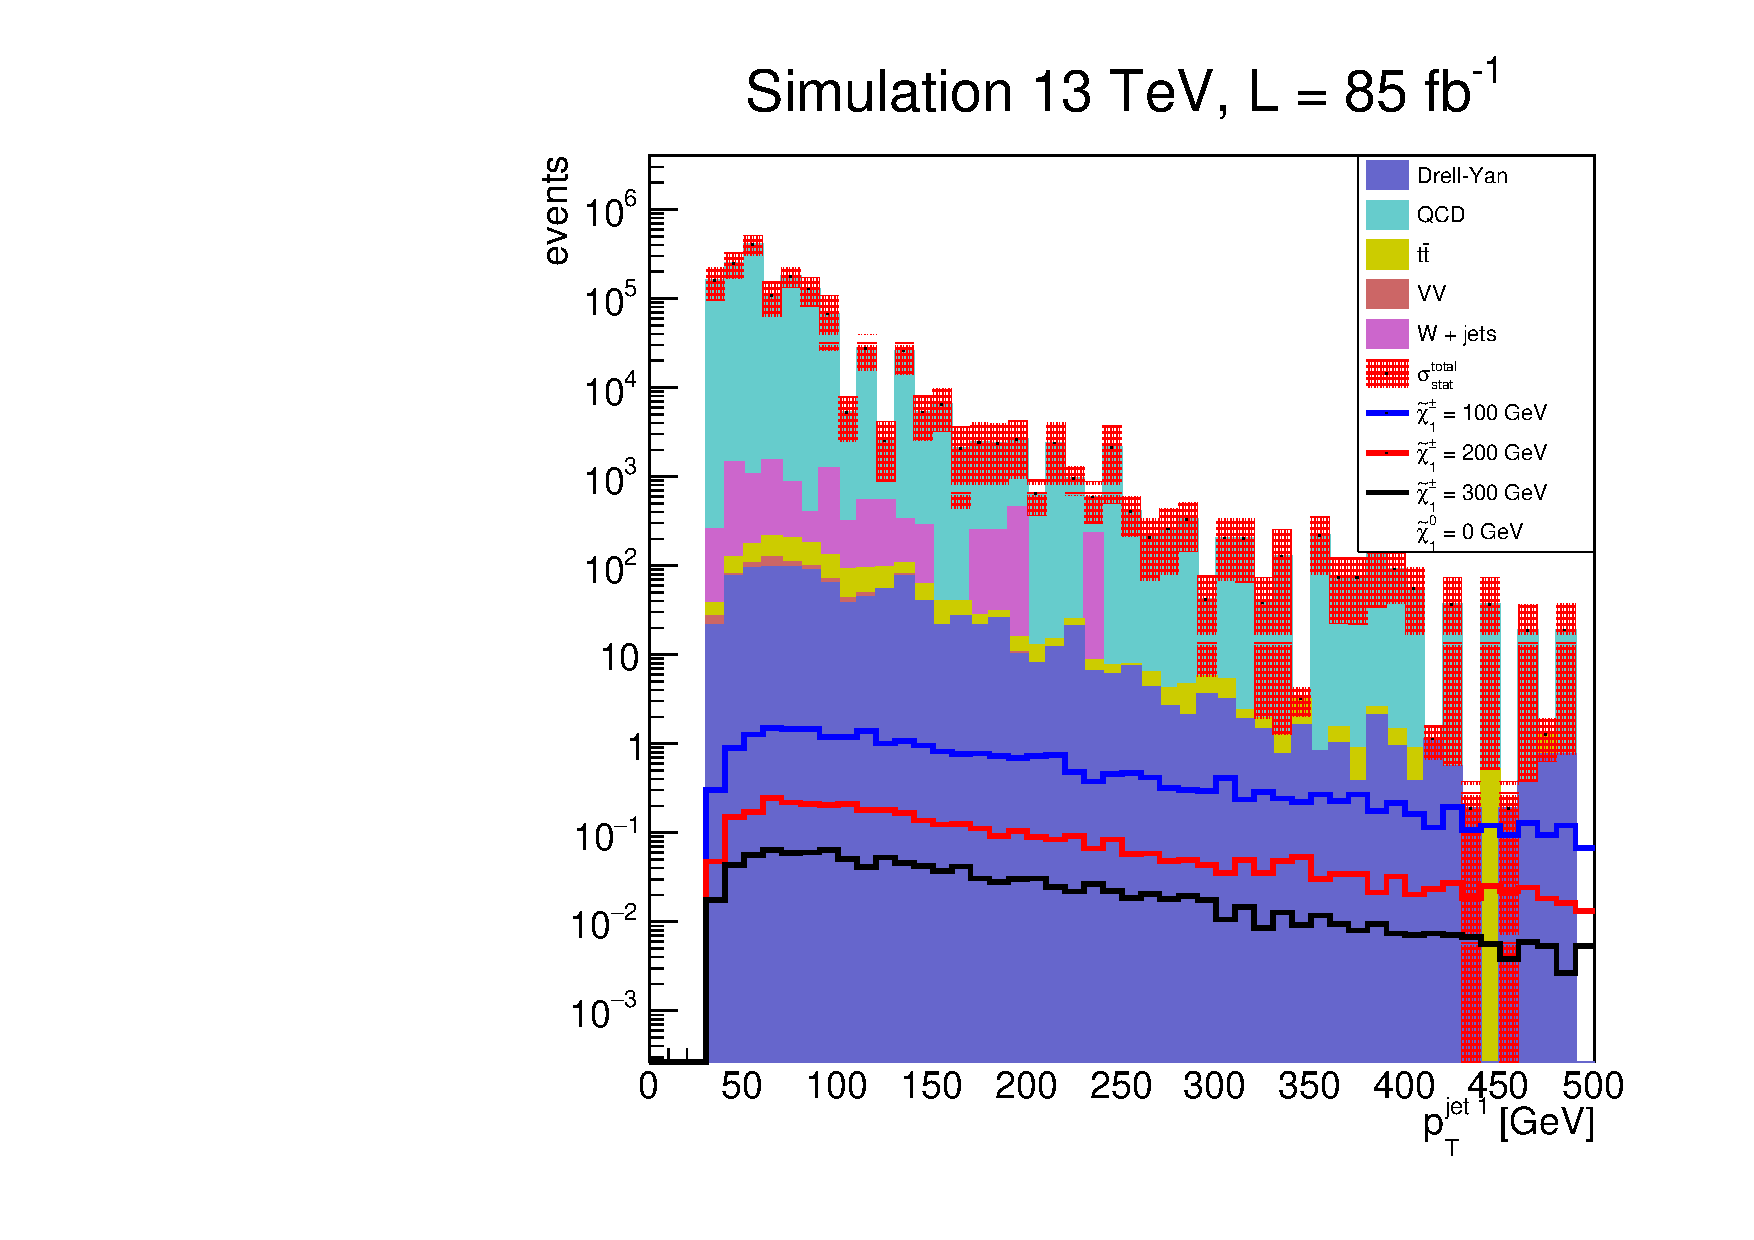
\includegraphics[width=0.5\textwidth]{analysis/pics/h_jet1pt_Taui2TightIso.pdf}
		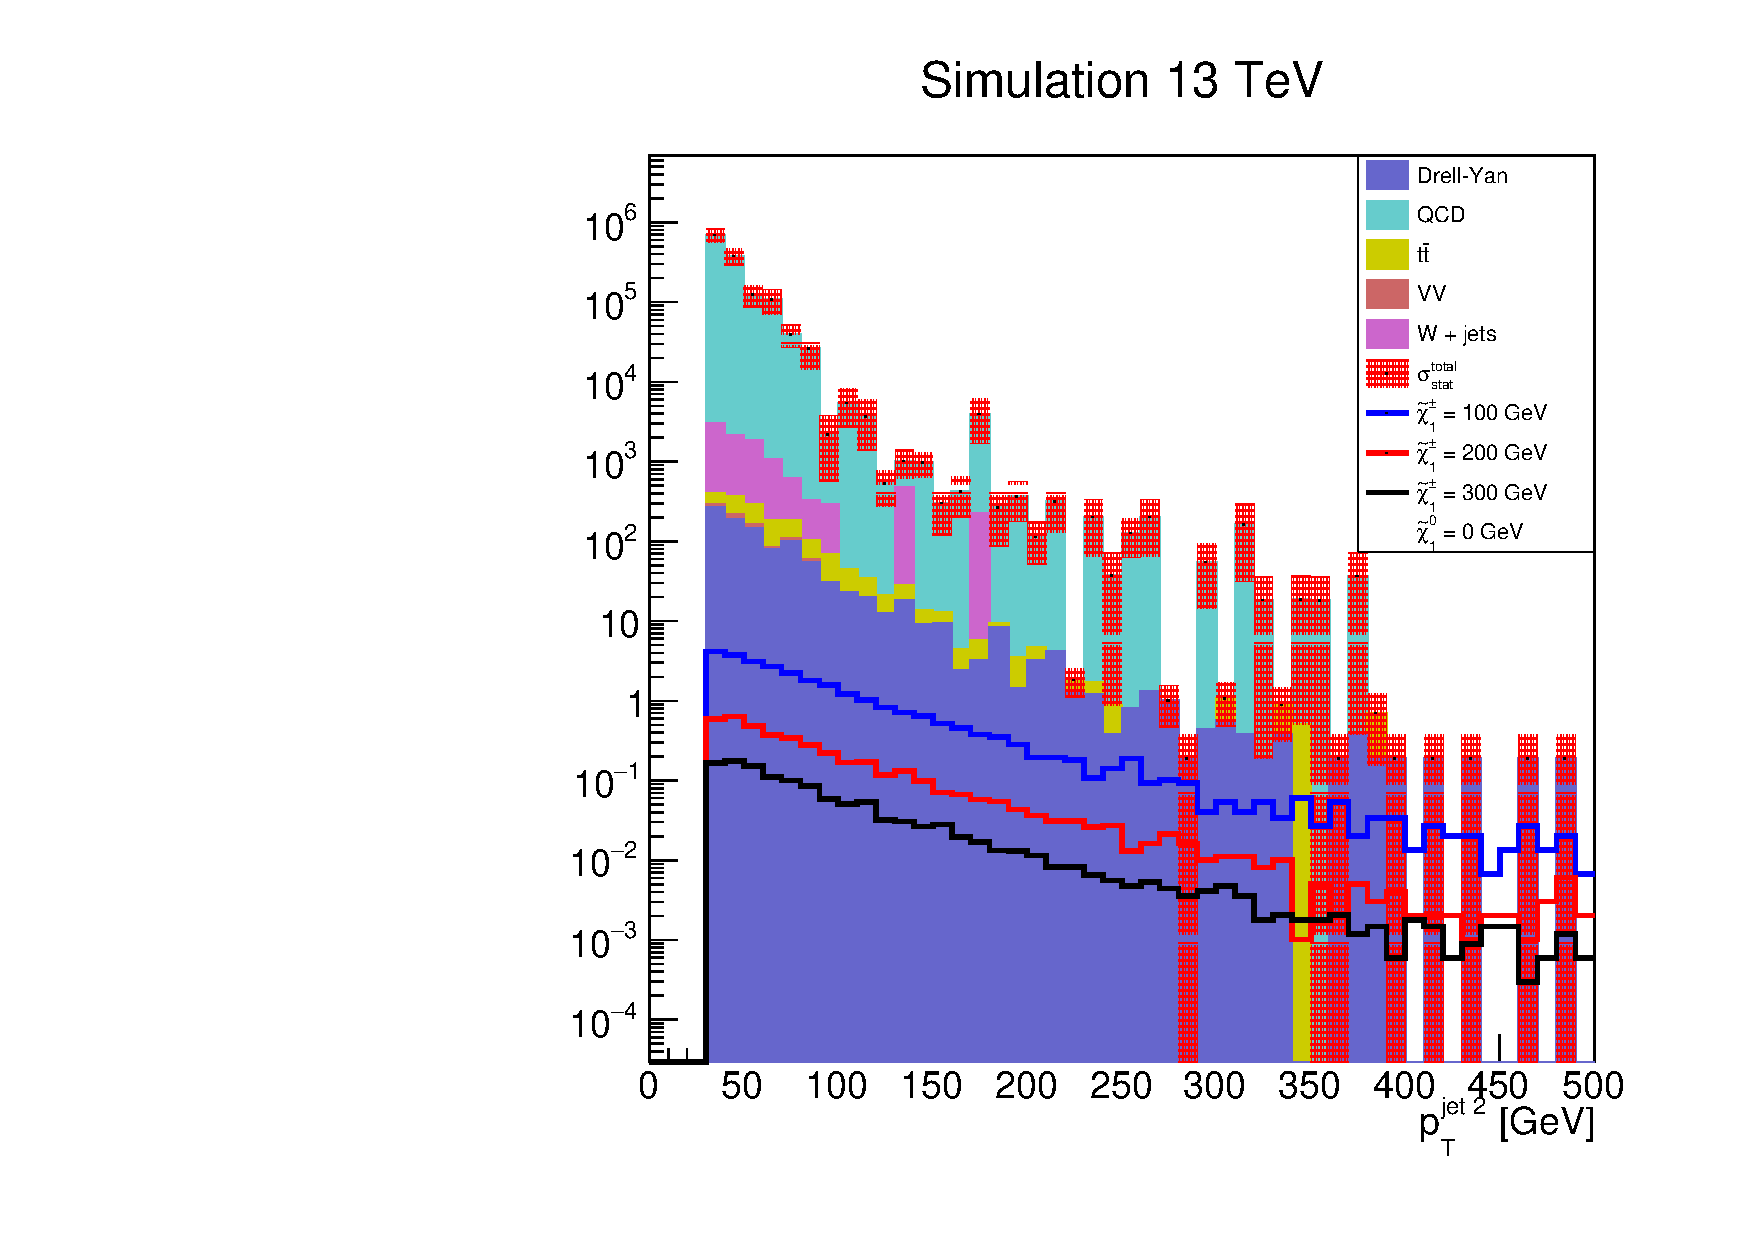
\includegraphics[width=0.5\textwidth]{analysis/pics/h_jet2pt_Taui2TightIso.pdf} 		
	\end{tabular}
	\caption{(Left) Leading jet \pt distribution and (Right) and second leading jet \pt distribution of selected signal and all MC background samples in signal region.}
	\label{fig::crplots3_Taui2TightIso_13tev_results}
\end{figure}

\begin{figure}[tbh!]
	\centering
	\begin{tabular}{cc}
		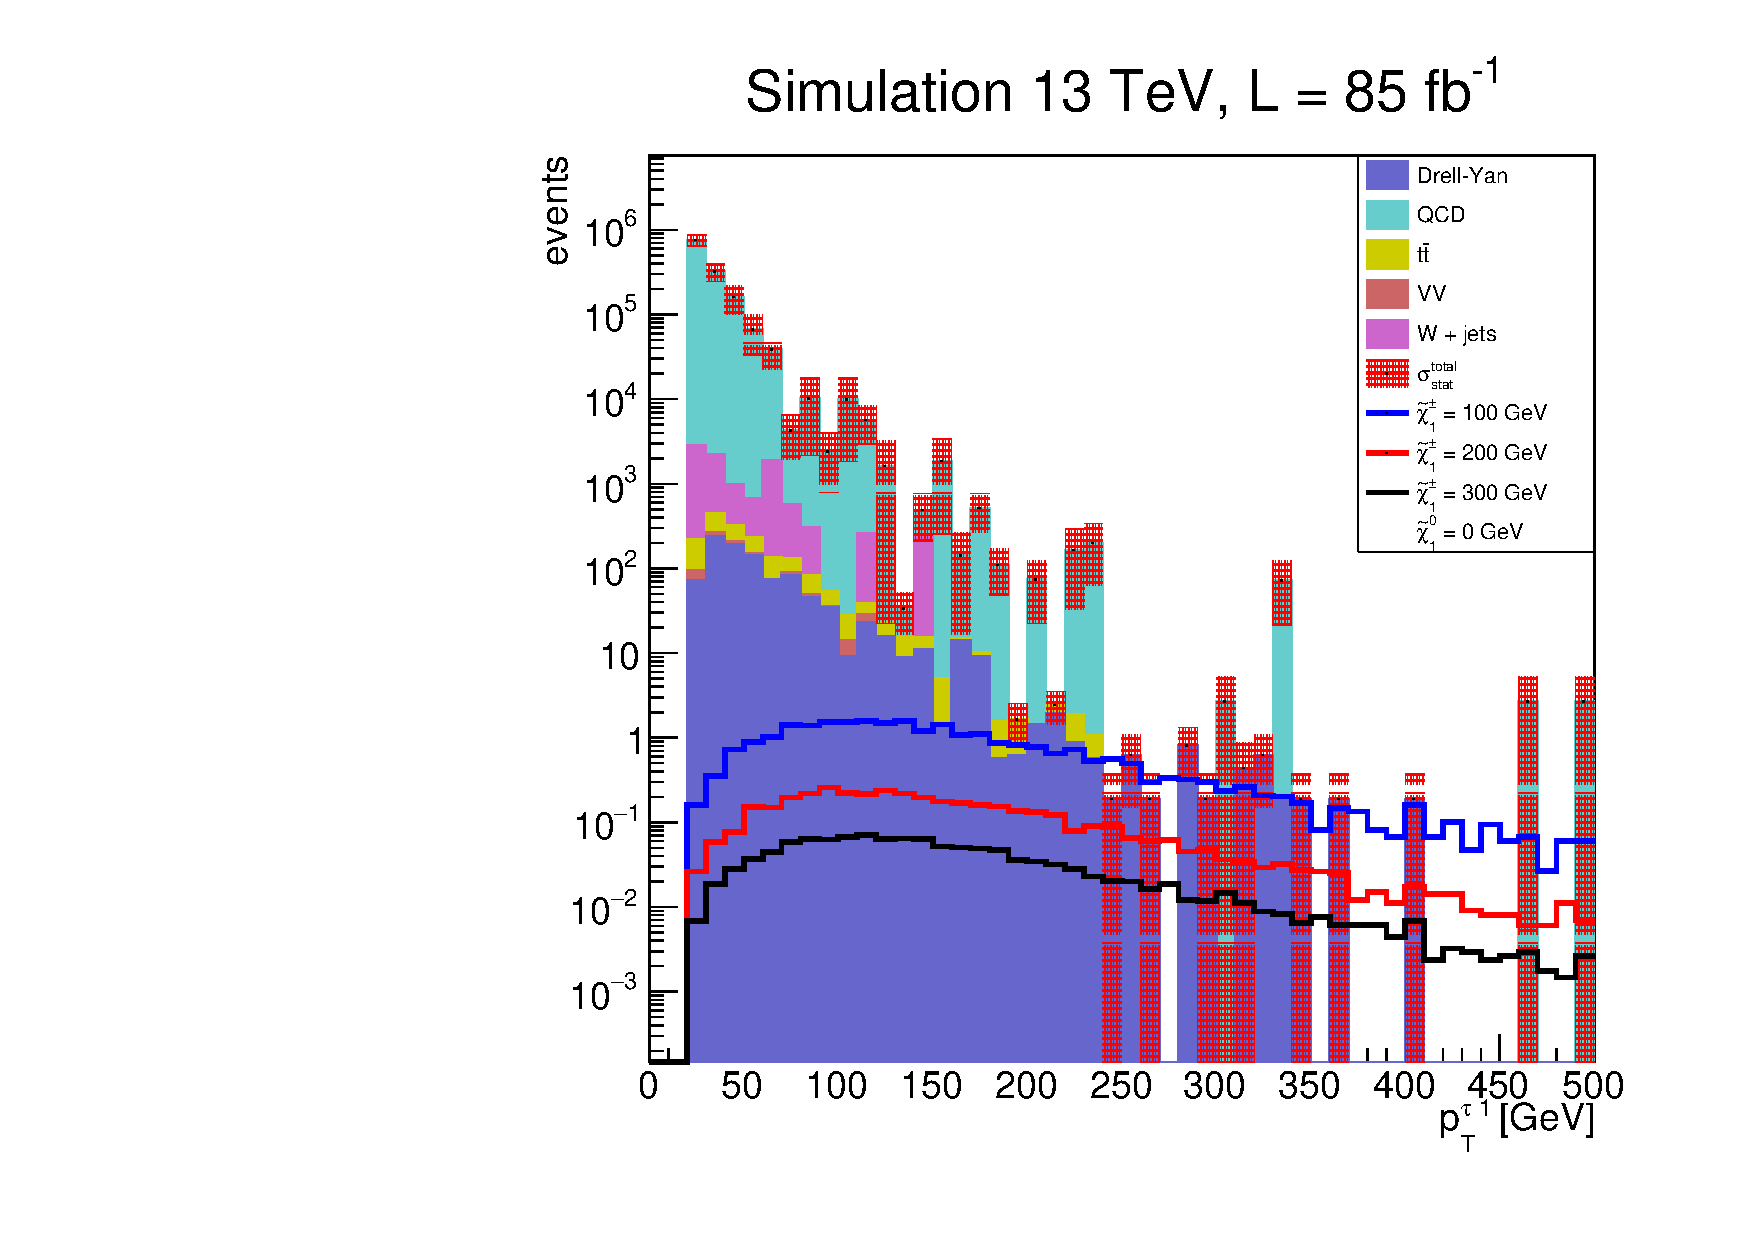
\includegraphics[width=0.5\textwidth]{analysis/pics/h_tau1pt_Taui2TightIso.pdf}
		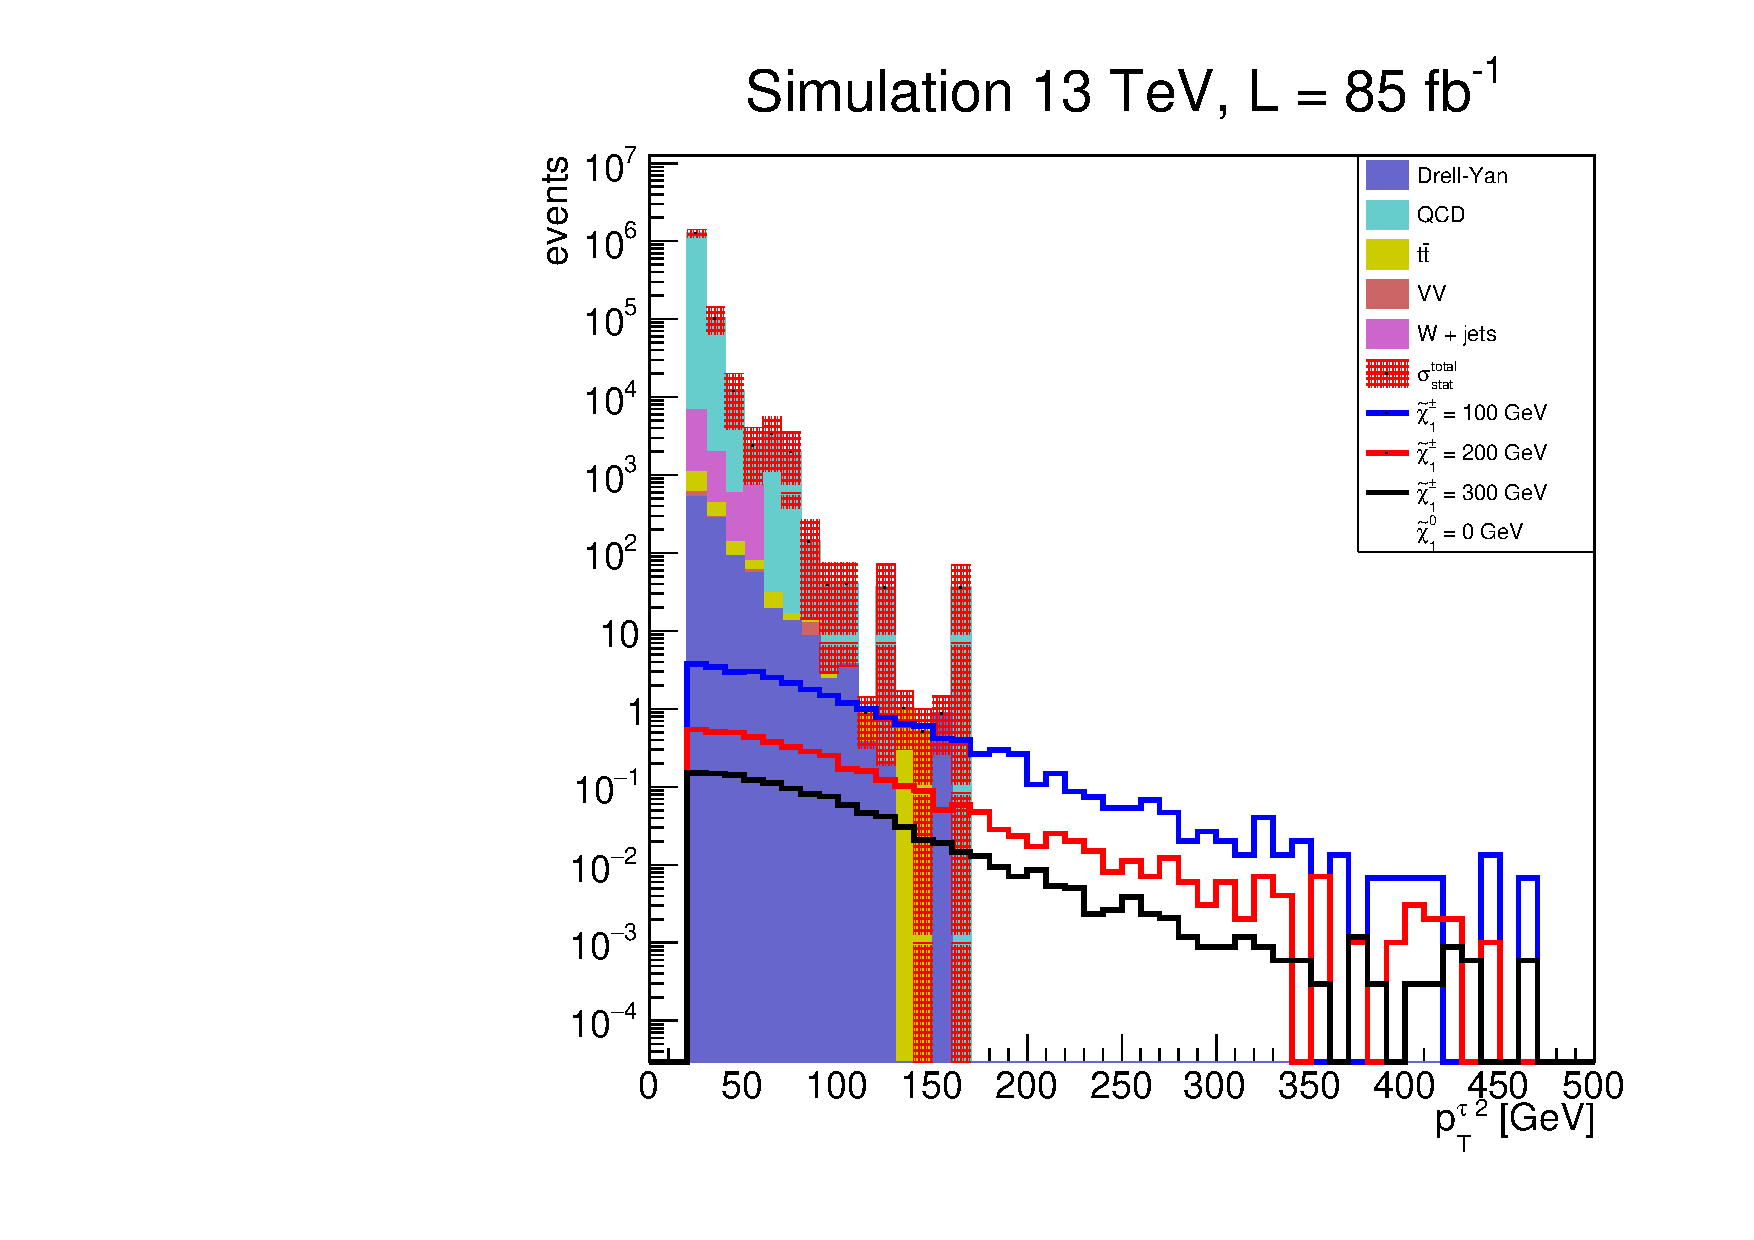
\includegraphics[width=0.5\textwidth]{analysis/pics/h_tau2pt_Taui2TightIso.pdf} 		
	\end{tabular}
	\caption{(Left) Leading \hadtau \pt distribution and (Right) and second leading \hadtau \pt distribution of selected signal and all MC background samples in signal region.}
	\label{fig::crplots4_Taui2TightIso_13tev_results}
\end{figure}


Each of the two-dimensional bins stores a $\sigma^{lim}_{sec}$ for the given $\pt(\hadtau)$ , \mjj and \met cuts setup. The most important input values to \autoref{eq::xsec_lim} are the signal efficiency $\epsilon^{signal}$, as defined in \autoref{eq::punzi_efficiency},  and the number of predicted background events $B$, as defined in \autoref{eq::qcdbgpred_13tev}. The remaining input values are the luminosity $L$ and the confidence level $a$. The predicted luminosity for the 13\tev Run \cite{Bruning:2002yh} is estimated between 75 and 100\invfb; for the purpose of this study its value has been set to $L = 85\invfb$. The corresponding value in terms of $\sigma$ with respect to a confidence level of 95\%  is $2.5$.

A full list of the study results is given as appendix in \autoref{sec::xseclim_results}. Similarly to what shown in the 8\tev analysis the cut over the $\pt(\hadtau)$ has an high impact on the signal efficiency $\epsilon^{signal}$; for an easier understanding of the final results this cut has been set to its allowed minimum of 20\gev.

The best cross-section limit scenario is given for a \charginopm and \neutralinotwo mass of 500\gev for the benchmark point assuming an uncompressed sparticles scenario and an average-\stau-mass assumption, as shown on \autoref{fig::xsec_lim_selected_results}. The cross-section limit minimum value is:

\begin{equation}
\sigma_{lim}^{min}\pm(stat.)\pm(MC syst.)\pm(VBF syst.) = 0.017\pm0.001^{+0.002 + 0.001}_{-0.002-0.000} [\text{pb}]
\label{eq::xsec_lim_best_result}
\end{equation}

for the optimal cuts of  $\pt(\hadtau) <  20\gev$,  $ \mjj< 500\gev $ and $\met < 250\gev$.

\begin{figure}[tbh!]
	\centering
	\begin{tabular}{cc}
		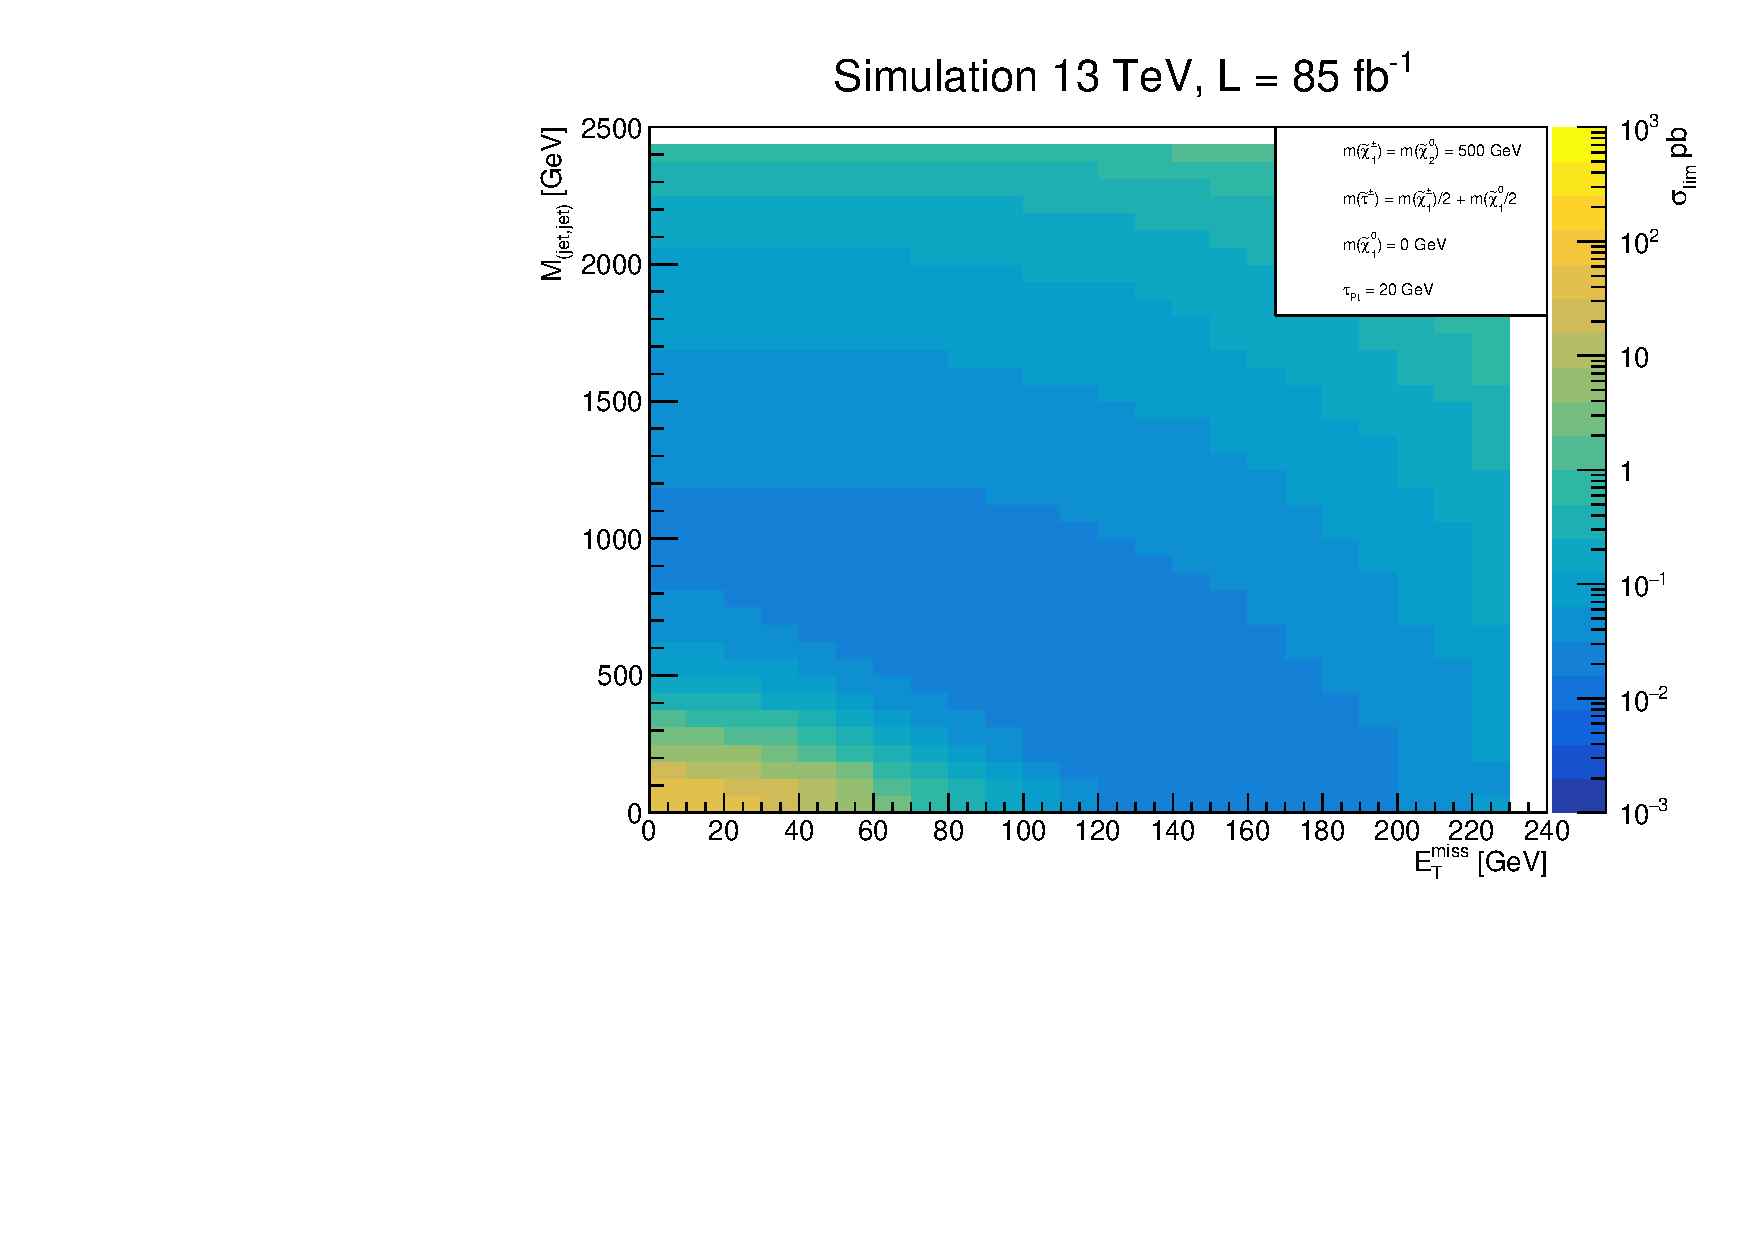
\includegraphics[width=0.75\textwidth]{analysis/pics/JetInvMass_vs_MET_xseclim_Chargino500_Stau250_LSP000_taupt20.pdf}
	\end{tabular}
	\caption{Cross section limit as function of $m_{jj}$ and \met for m(\charginopm) = m(\neutralinotwo) = 500 GeV,  m(\stau) = 250 GeV, and m(\neutralinoone) = 0 GeV and an offline selection on $\pt(\hadtau) <  20\gev$.}
	\label{fig::xsec_lim_selected_results}
\end{figure}

By comparing the 8\tev cross-section limit values with the ones at 13\tev it is possible to see that the previous analysis performs better in terms of limit setting as shown in \autoref{table::xseclim_7tev13tev_comparison}. The high statistical and systematic uncertainties shown for 13\tev are caused by the cut over the $\pt(\hadtau)$, which dramatically reduces the QCD statistics. It is worth to mention, however, that the 8\tev analysis has a selection which in general prevents the comparison in areas of the previously defined three-dimensional phase-space where the 13\tev analysis is meant to perform better.

\begin{table}
\begin{center}
\begin{tabular}{| c | c | c | }
	\toprule
	\multicolumn{3}{| c | }{For $\pt(\hadtau) <  45\gev$  $\met > $ 30, $\mjj>250~$\gev, m(\neutralinoone) = 50\gev} \\
	\midrule
	m(\charginopm) = m(\neutralinotwo)  & $\sigma_{lim}^{min}\pm(stat.)\pm(syst.)$ [pb] (8\tev) & $\sigma_{lim}^{min}\pm(stat.)\pm(syst.)$ [pb] (13\tev)\\
	\midrule
   100\gev &  $0.084\pm0.016^{+0.18}_{-0.01}$ & $0.60\pm0.69^{+1.62}_{-0.87}$  \\
   200\gev &  $0.14\pm0.02^{+0.03}_{-0.04}$ & $0.65\pm0.74^{+1.74}_{-0.94}$ \\
   300\gev &  $1.43\pm0.52^{+0.49}_{-0.38}$ & $1.19\pm1.39^{+3.2}_{-1.71}$  \\
	\bottomrule
\end{tabular}\caption{Cross-section limit comparison between the 8\tev analysis and the 13\tev sensitivity study. The chosen values corresponds to an identical selection and signal benchmark points. Cross section limit minimum reached at the given cuts for $\pt(\hadtau) <  45\gev$  $\met > $ 30, $\mjj>250~$\gev, m(\neutralinoone) = 50\gev.}
\label{table::xseclim_7tev13tev_comparison}
\end{center}
\end{table}

Another important result from this cross section limit study features the most important signal benchmark point among the ones available that originally gave reason to this analysis design, the one considering a compressed sparticles scenario and the average-\stau-mass assumption.  A comparison between the cross-section limit values coming from this study and the cross-section limit granted by the CMS collaboration \cite{bib:SUSYCrossSections13TeVn2x1wino_13tev} as function of the chargino \charginopm massis shown in \autoref{fig:xsec_confront_13tev}. Given the previously described setup, this analysis is capable of excluding models with chargino masses below $m(\charginopm) = 380\gev$. 

\begin{figure}[tbh!]
	\centering
	\begin{tabular}{cc}
		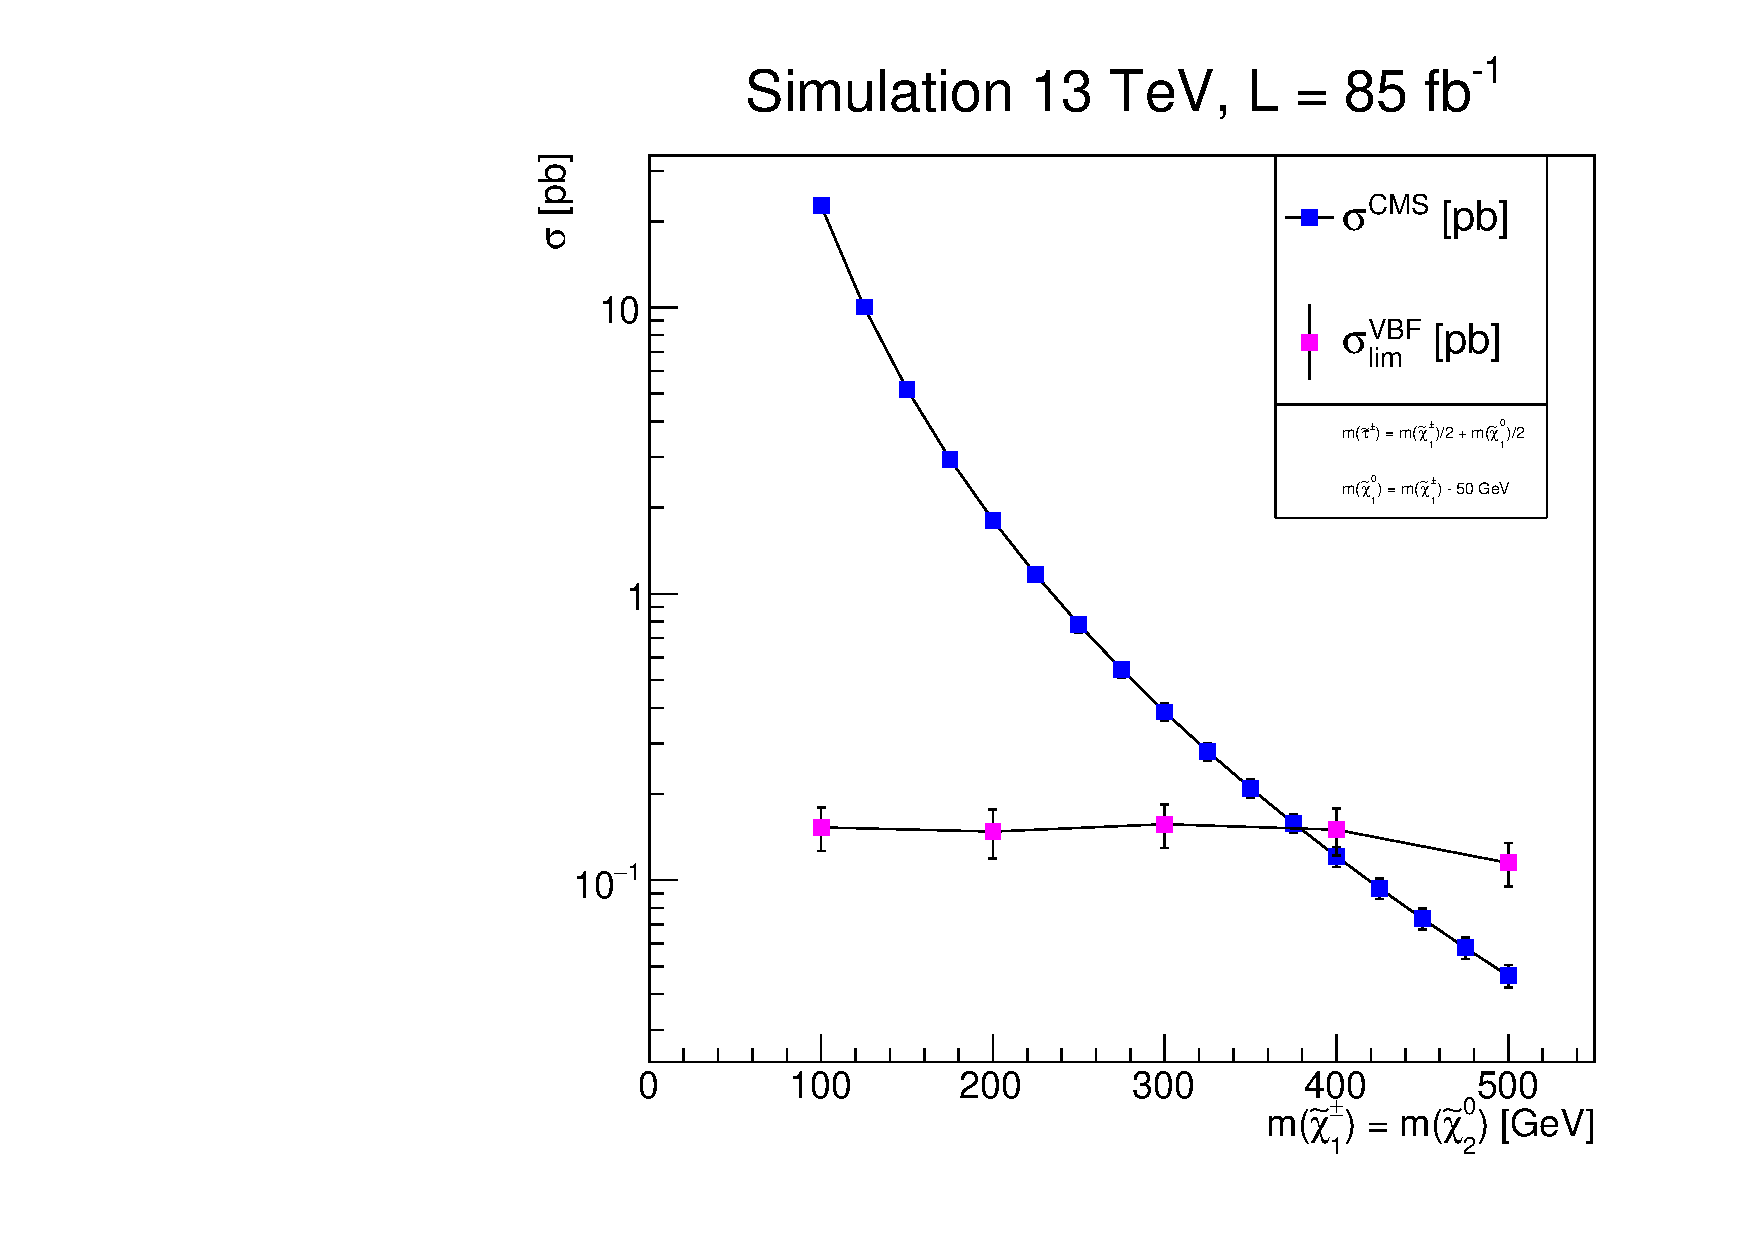
\includegraphics[width=0.75\textwidth]{analysis/pics/out_xsecmin_lspcomp_stauclose.pdf}
	\end{tabular}
	\caption{Comparison between the cross section limit given by this 13\tev study and official CMS cross sections calculated using the \texttt{resummino} code from B. Fuks et al with CTEQ6.6 and MSTW2008nlo90cl PDFs \cite{Fuks:2013vua}.}
	\label{fig:xsec_confront_13tev}
\end{figure}


To conclude the list of results shown in this chapter an additional study over this last signal benchmark point has been performed. The aim of this apply a more realistic event selection too see how strong is its impact over the cross section limit. In order to achieve that four different event selection scenarios has been considered. Those scenarios are meant to apply on top of the original event selection, described in \autoref{subsec::event_sel_13tev}, a stronger cut over the most important variable of the analysis. The first scenario simply adds a cut over the \pt of the \hadtau of 50 \gev. The second scenario adds a cut over \met of 200\gev. The third scenario combines the requirement of $\met > 150\gev$  with some cuts over the most important variables of the VBF part of the event such as $\mjj > 700\gev$, the angular distance between the two VBF jets candidates $|\Delta\eta(jet,jet)| > 3.6$ and their \pt set to 90\gev. The fourth and final scenario is similar to the third but requires a cut on  $\mjj > 1000\gev$ and removed any requirement over \met. For a better visualization those different scenarios are summarised the following way:

\begin{enumerate}
	\item \textbf{Cut scenario 1}: 
		\begin{itemize}
		\item $\pt(\hadtau) > 50\gev$;
	\end{itemize}

	\item \textbf{Cut scenario 2}: 
	\begin{itemize}
		\item 	$\met > 200\gev$;
	\end{itemize}

	\item \textbf{Cut scenario 3}: 
	\begin{itemize}
		\item $\met > 150\gev$,
		\item $\mjj > 700\gev$, 
		\item $|\Delta\eta(jet,jet)| > 3.6$,
		\item $pt (jet_{1},jet_{2}) = 90 GeV$;
	\end{itemize}
	
	\item \textbf{Cut scenario 4}: 			
	\begin{itemize}
		\item $\mjj > 1000\gev$, 
		\item $|\Delta\eta(jet,jet)| > 3.6$,
		\item $pt (jet_{1},jet_{2}) = 90\gev$.
	\end{itemize}
\end{enumerate}

Comparison between multiple cross section limits coming from the different cut scenarios and the official CMS cross section is shown in \autoref{fig:xsec_confront_cut_var13tev}.

\begin{figure}[tbh!]
	\centering
	\begin{tabular}{cc}
		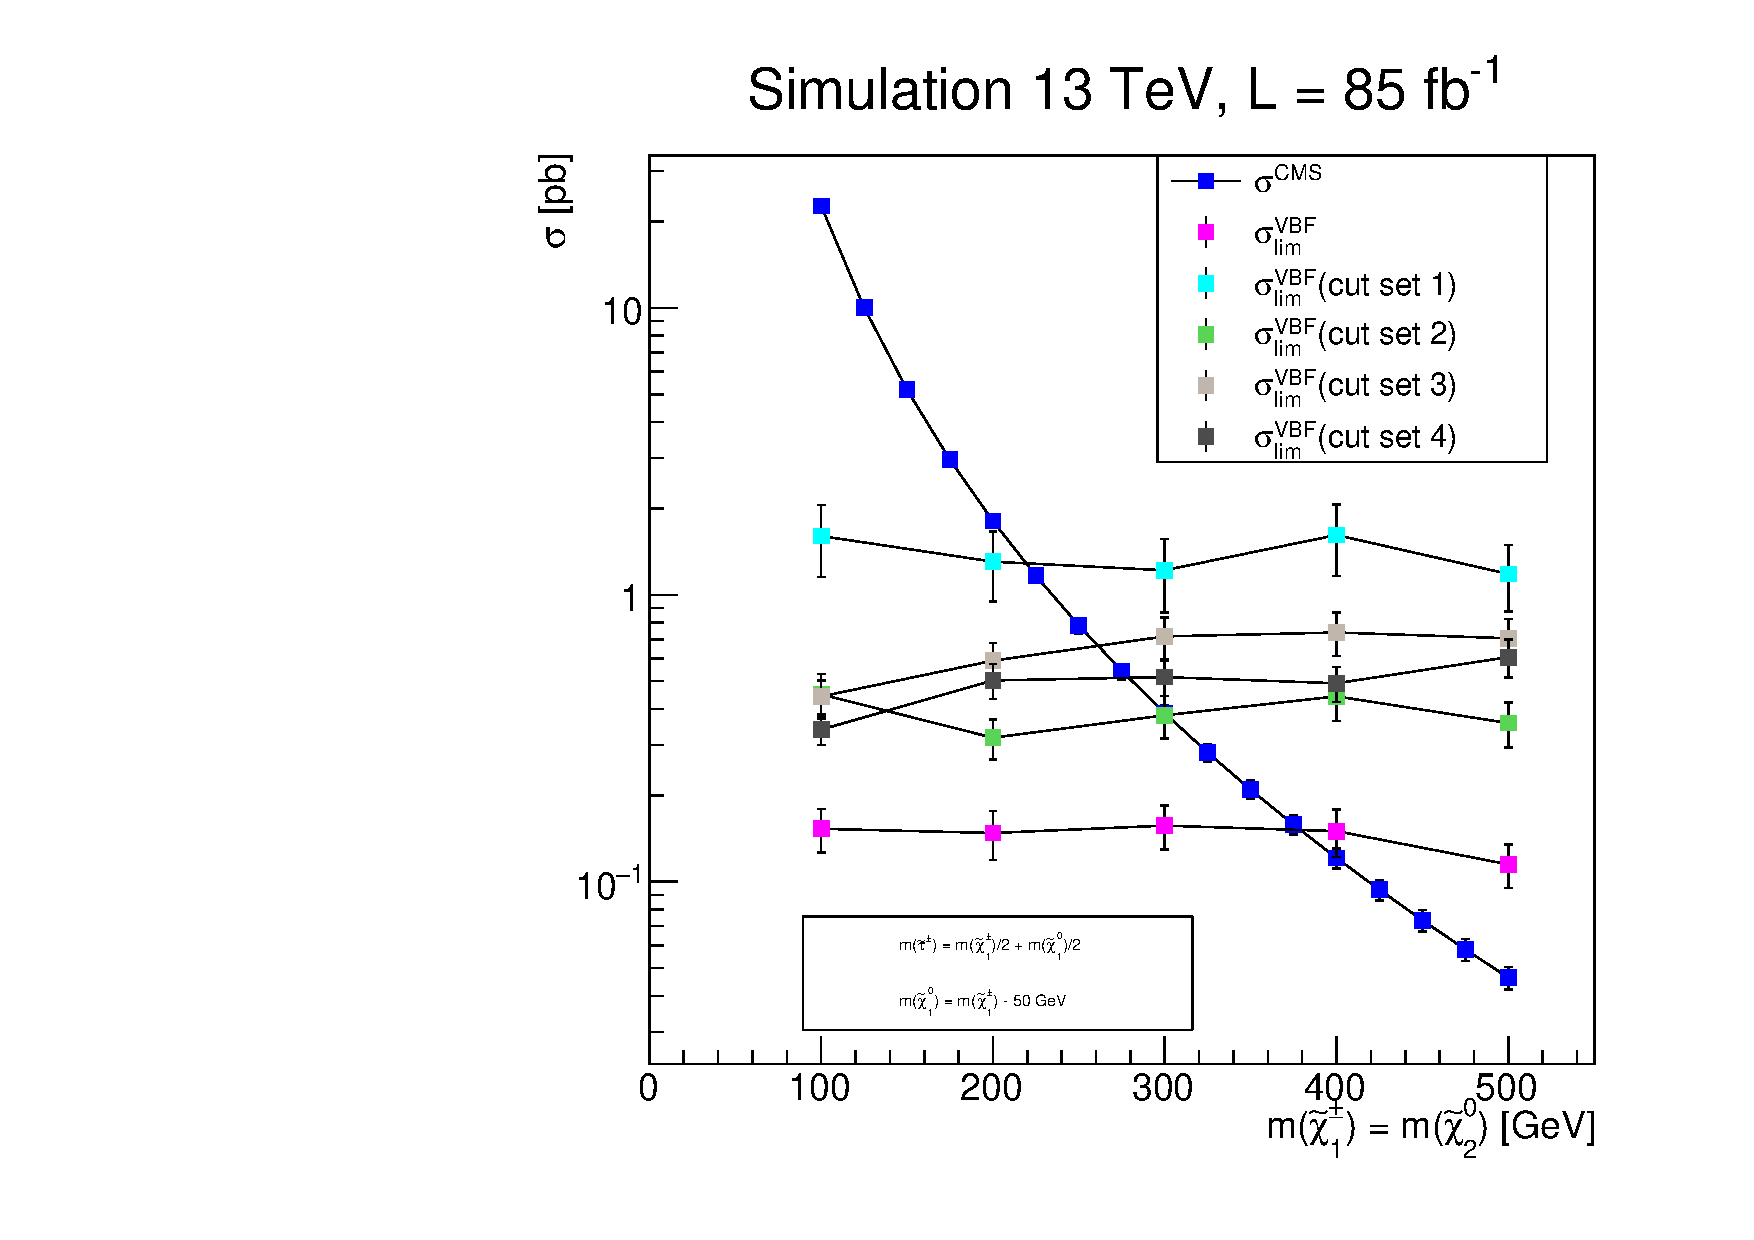
\includegraphics[width=0.75\textwidth]{analysis/pics/out_xsecmin_cutvar.pdf}
	\end{tabular}
	\caption{Comparison between multiple cross section limits given by different cut scenarios and the official CMS cross sections calculated using the \texttt{resummino} code from B. Fuks et al with CTEQ6.6 and MSTW2008nlo90cl PDFs \cite{Fuks:2013vua}.}
	\label{fig:xsec_confront_cut_var13tev}
\end{figure}

The correlation between signal efficiency and the selection over \pt(\hadtau) is once again confirmed by the drop on the cross section limit down to a chargino mass of 230\gev. The introduction of strong cut over \mjj combined with a requrement over \met (cut scenario 3) greatly impacts the limit setting by scaling down the original one down to a chargino mass of 270\gev. Similar performance in shown instead in the case where the cuts over those important variables get dissociated as shown for cut set number 2 and 4 with a cross section limit between a chargino mass of 280 and 300\gev.

